\documentclass{article}

%% Language and font encodings
\usepackage[french,english]{babel}
\usepackage[utf8x]{inputenc}
\usepackage[T1]{fontenc}
\usepackage{a4wide}

%% Sets page size and margins
\usepackage[a4paper,top=3cm,bottom=2cm,left=3cm,right=3cm,marginparwidth=1.75cm]{geometry}

%% Useful packages
\usepackage{amsmath}
\usepackage{graphicx}
\usepackage{caption}
\usepackage{multicol}
\usepackage[colorinlistoftodos]{todonotes}
\usepackage[colorlinks=true, allcolors=blue]{hyperref}

\title{M1 - Rapport Développement Mobile}
\author{LARUE Sebastien et CLAIN Jonathan, M1 Informatique}
\date{05/11/2018}

\begin{document}

\maketitle
\begin{abstract}
\Large
Dans le cadre de l'UE obligatoire développement mobiles, il est demandé de concevoir un jeu de notre choix sur la plate-forme Android et iOS. Dans ce cadre, nous avons travaillé en binôme pour réussir à coder au mieux le projet.\\
A cet effet, nous avons combiné notre temps, volonté et motivation, ainsi que nos capacités en informatique pour pouvoir réaliser au mieux ce projet qui nous tenait à cœur.\\
Nous avons dû surmonter et pallier avec nos erreurs et faiblesses pour concevoir et répondre aux cahier des charges ainsi que pour offrir aux utilisateurs le jeu le plus attractifs et distrayants possible.\\
A terme de quelques semaines de travail, nous avons donc réussi à mettre en place ce projet, qui répond au mieux aux demandes du cahier des charges.\\

\end{abstract}

\newpage
\part*{Introduction}
\Large
Le jeu Miaou Aventures, en accord avec les cahiers des charges proposés par le professeur de développement mobiles, a donc été réalisé sur Android et sur iOS. Nous avons fait en sorte que nos jeux soient semblables en tout point de vue.\\
Nous nous attellerons donc à vous présenter les différentes ficelles de sa conceptions que ce soit, d’abord, à travers la version Android puis, dans un second temps, celle d’iOS.

Afin de réaliser ce projet, différents sites et forums nous ont été utiles tels que: \cite{AndroidStudio}, \cite{Apple}, \cite{OpenClassroom}, \cite{RayWenderlich} et \cite{Youtube}

\section{Description}
Miaou Adventures s'inspire du principe et des modalités traditionnels des 'runners', à savoir encourager l'utilisateur à toujours dépasser son meilleur score. L'objectif est simple: guider le chat Miaou et son vaisseau intersidérale vers des territoires inconnus et à travers une tempête d'astéroïdes mortelles. Il s'agit d'un jeu amusant et addictif, et surtout accessible à tous les âges. Le jeu s'arrête seulement lorsque le vaisseau de Miaou est détruit .\\
Les deux versions encouragent le joueur à poursuivre sa quête et ses aventures à travers l'hyperespace grâce à un thème futuriste et esthétique. Les nombreuses autres options comme la localisation et l'appareil photo rajoutent un plus non négligeable fondamental dans l'attractivité du jeu. 
Il s'agit de fonctionnalités novatrices dans les jeux de 'runners' et qui nous permettraient de nous démarquer. 

\newpage
\section{Architecture générale}
\subsection{Android}
%Completer par JClain
Cette partie du rapport sera consacrée a présenter l'architecture générale de la version Android de notre projet.\\
La version Android a été réalisé sur Android Studio en langage Java par Jonathan Clain.

\subsubsection{MainActivity.java}
C'est dans cette classe que l'on met en place le menu de notre jeu. En effet, le menu se compose de plusieurs boutons dont le bouton 'Play', 'Score', 'Son' et 'Réinitialiser Score'. De plus cette classe coordonne les évènements sur les boutons. L'utilisateur peut ainsi lancer le jeu, visualiser le score, activer ou désactiver le son et réinitialiser le score.

\subsubsection{GameActivity.java}
C'est l'une des classes les plus importantes. C’est là que l’on gère les activités de notre jeu tel que le lancement, la mise en pause et enfin l’arrêt du jeu.
Premièrement, nous avons la méthode onResume() qui va tout simplement lancer le jeu. Ensuite nous avons  la méthode onPause(), elle permet de mettre le jeux en pause.
Aussi c'est dans cette classe que l'on initialise la vue du jeu "Gameview" que l'on abordera par la suite. Une bannière en haut de l'écran est aussi intégrée.
Elle est composée de l'affichage du score, d'un bouton retour, pause et reset. L'utilisateur peut donc effectuer ces différentes actions lorsque le jeu est en exécution. 

\subsubsection{GameView.java}
La classe GameView hérite donc de Surfaceview et intègre l'interface  SurfaceHolder.Callback. En effet, nous avons besoin de créer une surface dédiée afin de déssiner.
On a également besoin de plusieurs éléments pour dessiner: un Canvas, un Bitmap et un Paint.
C'est dans cette classe que l'on va instancier les éléments de notre jeu, puis les afficher en utilisant les fonctions de dessin.

\newpage
Afin d'afficher le gameView dans notre "scene.xml" il faut donc lier ce dernier en tant que vue. 
\begin{verbatim}
    <com.example.clain.miaou.GameView
            android:id="@+id/SurfaceView01"
            android:layout_width="match_parent"
            android:layout_height="match_parent" />
    }
\end{verbatim}

\begin{center}
    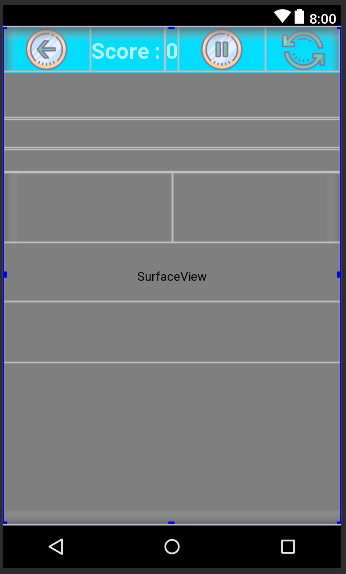
\includegraphics[scale = 0.7]{images/gameview.PNG}
    \captionof{figure}{GameView}
\end{center}

\subsubsection{Items.java}
Dans cette classe, nous avons ajouté les différents sprites du jeu tels que la météorite, la pièce et le héros. Lors de l'instanciation, la position de ces derniers sont initialisées a l'aide du constructeur qui récupère en paramètres le contexte de l'application et les dimensions de l'écran. Une méthode Update permet le déplacement de ces sprites lorsque le jeu est en exécution. Enfin, des 'getters' permettent de récupérer les positions et les bitmaps et enfin des 'setters' afin de les modifier.

\newpage
\subsubsection{Hero.java}
La classe hero permet d'ajouter le personnage principal dans le jeu. Tout d'abord, nous avons un constructeur. On récupère ainsi l'image du héros et on initialise sa position initiale. Une méthode moveHero permet de mettre à jour la position du héros dans le gameView lorsque le jeu est en exécution.\\

De plus, le déplacement du héros se fait en utilisant les capteurs du smartphone, l'accéléromètre. Ainsi, la classe implémente un SensorEventListener.

\begin{verbatim}
    manager = (SensorManager) context.getSystemService
    (Service.SENSOR_SERVICE);
        if (manager != null) {
            mAccelerometer = manager.getDefaultSensor
            (Sensor.TYPE_ACCELEROMETER);
        }
\end{verbatim}

Deux méthodes permettent d'activer ou désactive le déplacement:

\begin{verbatim}
     public  void activerDeplacement(){
        accelSupported = manager.registerListener
        (this, mAccelerometer, SensorManager.SENSOR_DELAY_GAME);
    }

    public void desactiverDeplacement(){
        if(accelSupported){
            manager.unregisterListener(this,mAccelerometer);
        }
    }
\end{verbatim}

\subsubsection{ScoreView.java}
En démarrant le jeu pour la première fois, le score est à 0. A la fin de chaque de partie le meilleur score est sauvegardé. La sauvegarde s’effectue à travers le ’SharedPreferences’. Les SharedPreferences sont des espaces de stockage propres à chaque application Android.

\newpage
\subsubsection{MapsActivity.java}
Afin de répondre aux demandes du cahier des charges, l’intégration de la géo-localisation était nécessaire. Le MapsActivity permet à l’application d’accéder à Google Maps et ainsi de déterminer la position actuelle du joueur. 

\subsubsection{Internationalisation}
L'internationalisation sur Android est relativement simple:
\begin{center}
    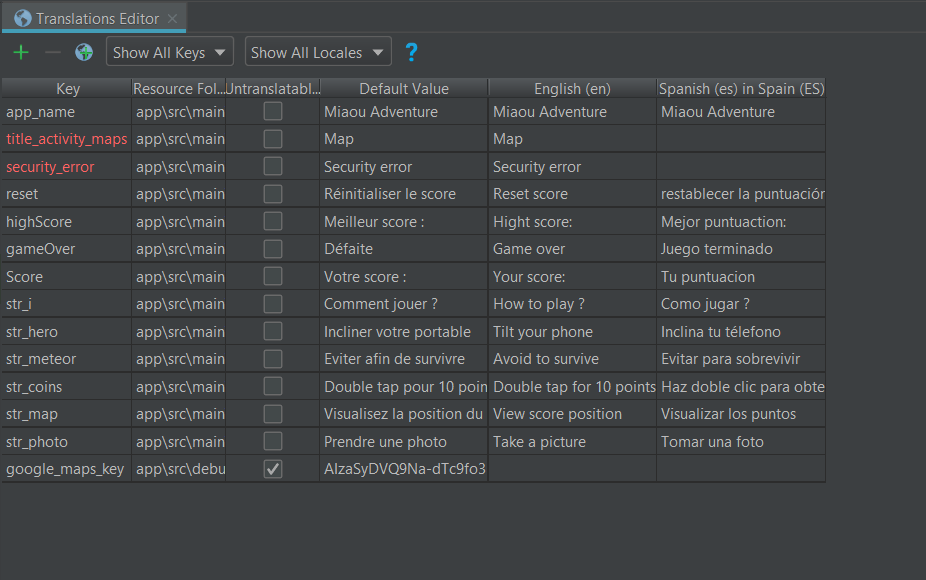
\includegraphics[scale = 0.7]{images/translate.PNG}
    \captionof{figure}{Internationalisation}
\end{center}


\newpage
\subsection{iOS}
Cette partie-ci est destinée à la présentation de l'architecture générale de la version iOS de notre projet.\\
La version iOS a été réalisé sur Xcode en langage Swift avec SpriteKit par Sebastien Larue.

\subsubsection{MainMenuScene.swift}
C'est dans ce fichier que nous mettons en place le menu de notre jeu. Ce dernier se compose de divers boutons dont le bouton 'Play', 'Score' et 'Son'. C'est donc ce fichier qui coordonne les évènements sur les boutons, qui vont nous permettre de lancer le jeu, de visualiser le score et d'activer ou désactiver le son.

\subsubsection{GameElements.swift}
Ce fichier regroupe tous les éléments du jeu crées sous forme de fonctions. Ces fonctions sont ensuite appelées dans dans le GamePlayScene.swift.\\
Le code ci-dessous est une fonction qui permet de créer un bouton retour et de le positionner sur l'interface: 
\begin{verbatim}
    func createBackButton(){
        backButton = SKSpriteNode(imageNamed: "back")
        backButton.position = CGPoint(x: self.frame.width/12, 
        y: self.frame.height * 0.95)
        backButton.zPosition = 4
        self.addChild(backButton)
    }
\end{verbatim}

\subsubsection{GamePlayScene.swift}
C'est le fichier principale de notre projet. Il coordonne l'ensemble des actions de notre jeu. On retrouve dans un premier la déclaration et l'instanciation des variables du jeu. Le code fait appel à toutes nos fonctions du fichier GameElements.swift. On retrouve aussi d'autres codes qui gèrent chaque évènement sur les boutons, la collision entre les sprites et le geste courant.\\

\newpage
Ci-dessous on retrouve le code qui permet d'ajouter un geste courant sur le 'view' du jeu, le double tap: 
\begin{verbatim}
    let tap = UITapGestureRecognizer(target: self, 
    action: #selector(doubleTapped))
        tap.numberOfTapsRequired = 2
        tap.numberOfTouchesRequired = 1
        view.addGestureRecognizer(tap)
\end{verbatim}

\subsubsection{ScoreScene.swift}
En démarrant le jeu pour la première fois, le score est à 0. A la fin de chaque de partie, le meilleur score est sauvegardé. La sauvegarde s'effectue à travers le 'UserDefaults'. C'est une classe qui permet de stocker des données de petite taille. \\
Dans un premier temps, on sauvegarde le score à la fin de la partie si il est supérieur à 0 ou du meilleur score précédent: 
\begin{verbatim}
    let defaults = UserDefaults.standard
    let hscore = defaults.integer(forKey: "highestScore")
    if hscore < score{
        defaults.set(score, forKey: "highestScore")
    }                    
\end{verbatim}

Dans un second temps, on recupère le score pour l'afficher dans l'intreface de score: 

\begin{verbatim}
    let defaults = UserDefaults.standard
    let highestScore = defaults.object(forKey: "highestScore")
\end{verbatim}

\subsubsection{MapView.swift}
Afin de répondre aux demandes du cahier des charges, l'intégration de la géo-localisation était nécessaire. Le MapView.swift permet à l'application d'accéder à l'Apple Maps. Dans un premier temps, il fallait d'abord faire appel à la classe MKMapView. Cette classe nous permet d'afficher la map sur l'écran.\\
Dans un second temps, il fallait déterminer la position actuelle du joueur. Pour cela, il fallait faire appel à la classe CCLocationManager.\\
On a ajouté une épingle sur la position actuelle de l'utilisateur avec en légende les coordonnées géographiques.

\newpage
\subsubsection{ViewController.swift}
Le ViewController.swift va nous permettre d'accéder à l'appareil photo, de prendre une photo et de la sauvegarder. Pour cela, on utilise la classe UIImagePickerController.\\
Voici le code qui va nous permettre de sauvegarder une photo dans la librairie: 
\begin{verbatim}
     @IBAction func onSaveButton(_ sender: Any) {
        guard let selectedImage = imageView.image else {
            print("Image not found!")
            return
        }
        UIImageWriteToSavedPhotosAlbum(selectedImage, self, #selector
        (image(_:didFinishSavingWithError:contextInfo:)), nil)
    }
\end{verbatim}

\subsubsection{Localizable.strings}
Afin de rendre le jeu disponible en francais et en anglais, nous avons fait appel au fichier Localizable.strings. A ce dernier, on ajoute les données de traduction sous formes de 'Key values'.\\
Vous pouvez voir ci-dessous un exemple de l'internationalisation dans notre application.

\begin{center}
    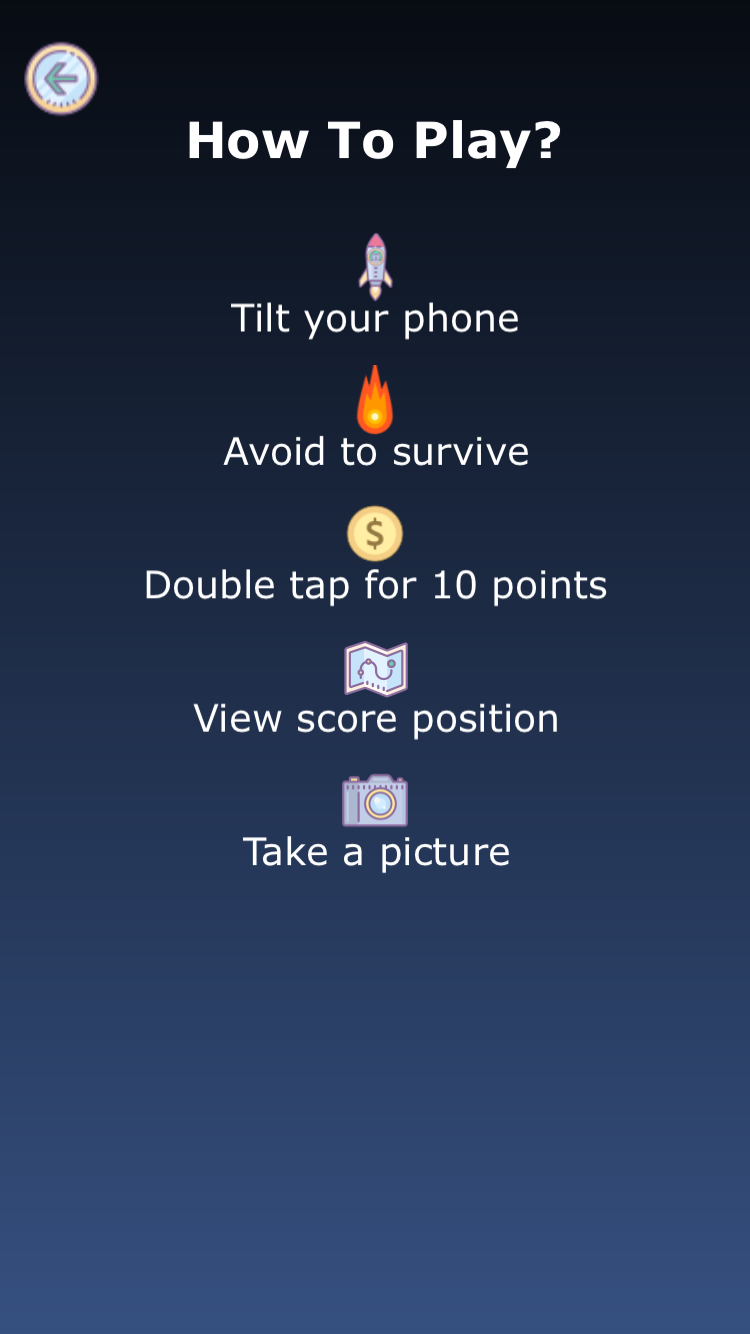
\includegraphics[scale = 0.2]{images/iOS_en.PNG}
    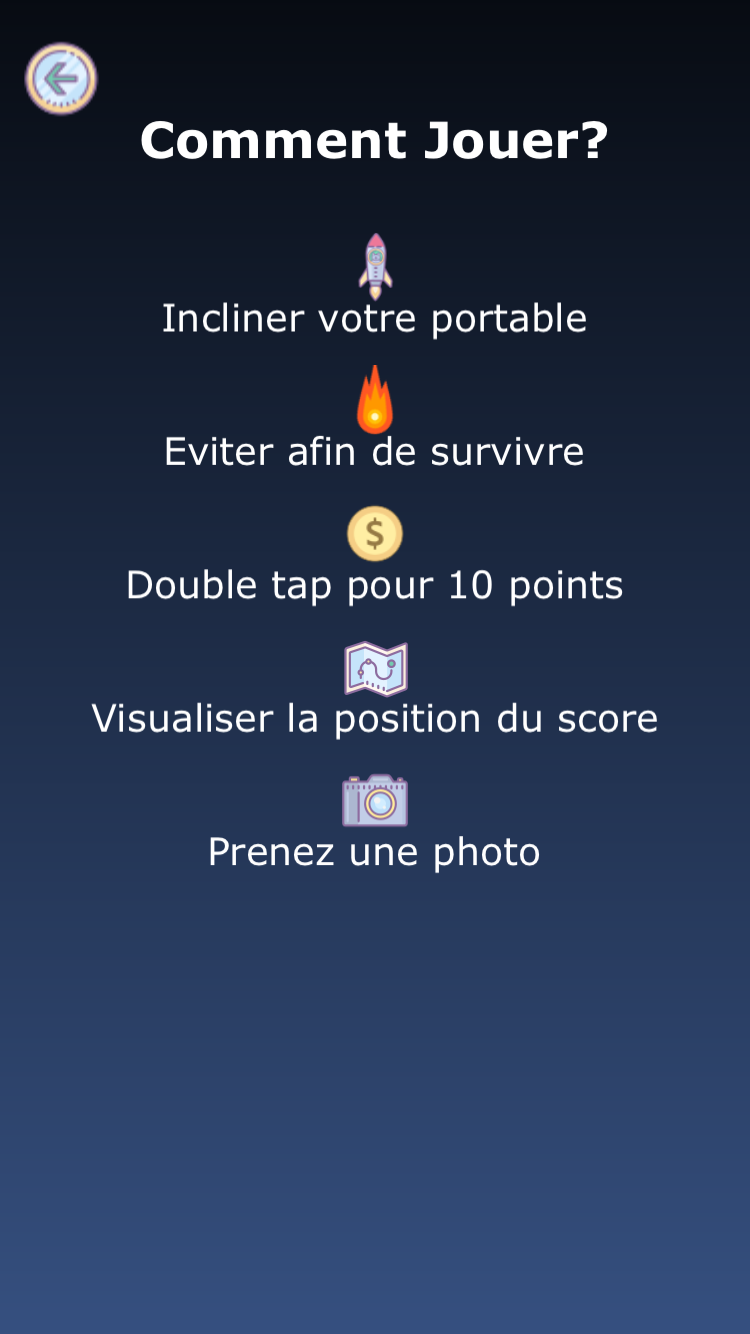
\includegraphics[scale = 0.2]{images/iOS_fr.PNG}
    \captionof{figure}{Gauche: English et Droite: Français}
\end{center}

\newpage
\section{Interfaces: Android et iOS}

Miaou Adventures se compose des interfaces suivantes:
\begin{multicols}{2}
\begin{itemize}
 \item Un menu de jeu
 \item L'interface de score
 \item L'interface de jeu
 \item L'interface de géo-localisation
 \item L'appareil photo
 \item L'interface de jeu
\end{itemize}
\end{multicols}

\subsubsection{Le menu de jeu}
Le menu nous offre un aperçu du thème du jeu. Il vous propose différentes fonctionnalités: démarrer une nouvelle partie, de nous montrer le meilleur score, de le réinitialiser, nous donner des indications sur le fonctionnement du jeu ou le mettre en mode sourdine. On peut également constater une bannière publicitaire.

\subsubsection{L'interface de score}
A la fin de chaque partie, il existe deux possibilités: soit le meilleur score qui n'a pas été dépassé au cours de la dernière partie s'affiche, soit c'est le nouveau record atteint qui s'affiche.\\

Voir ci-dessous les images correspondantes à l'interface menu et score du jeu:

\begin{center}
    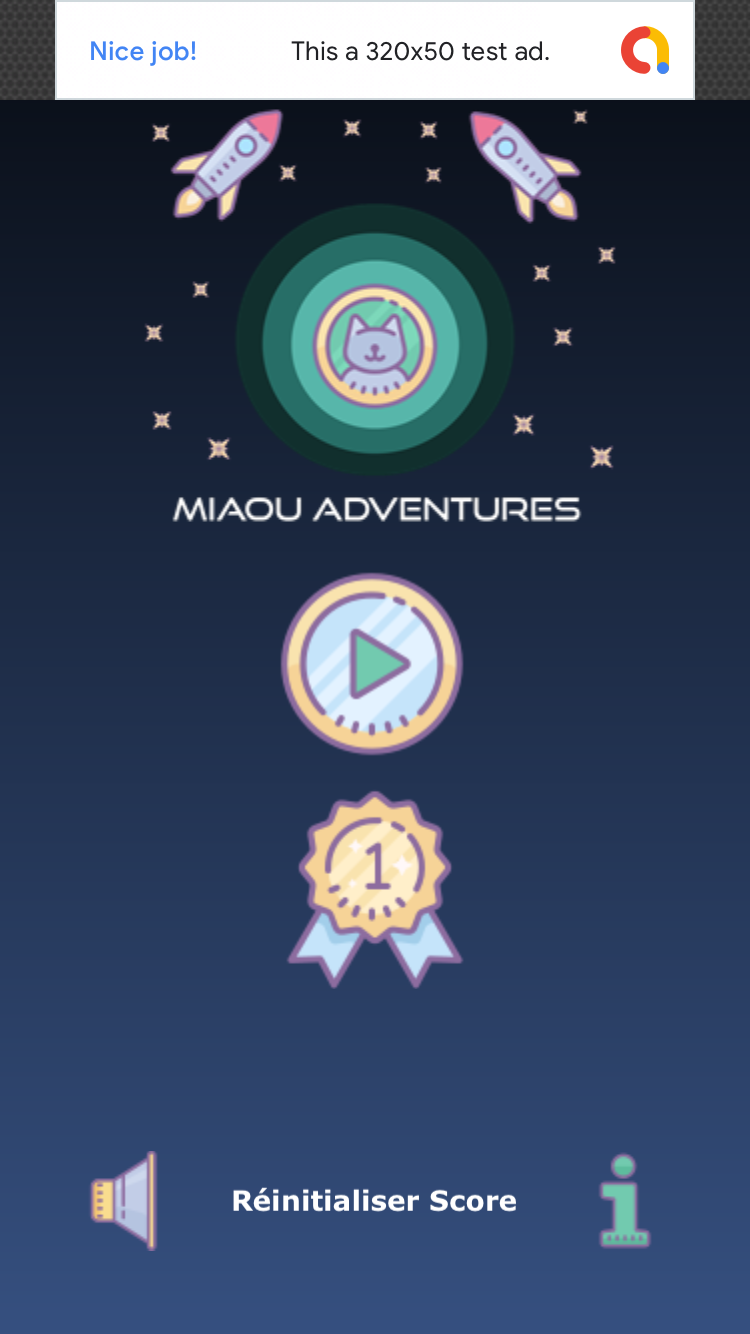
\includegraphics[scale = 0.18]{images/iOS_1.png}
    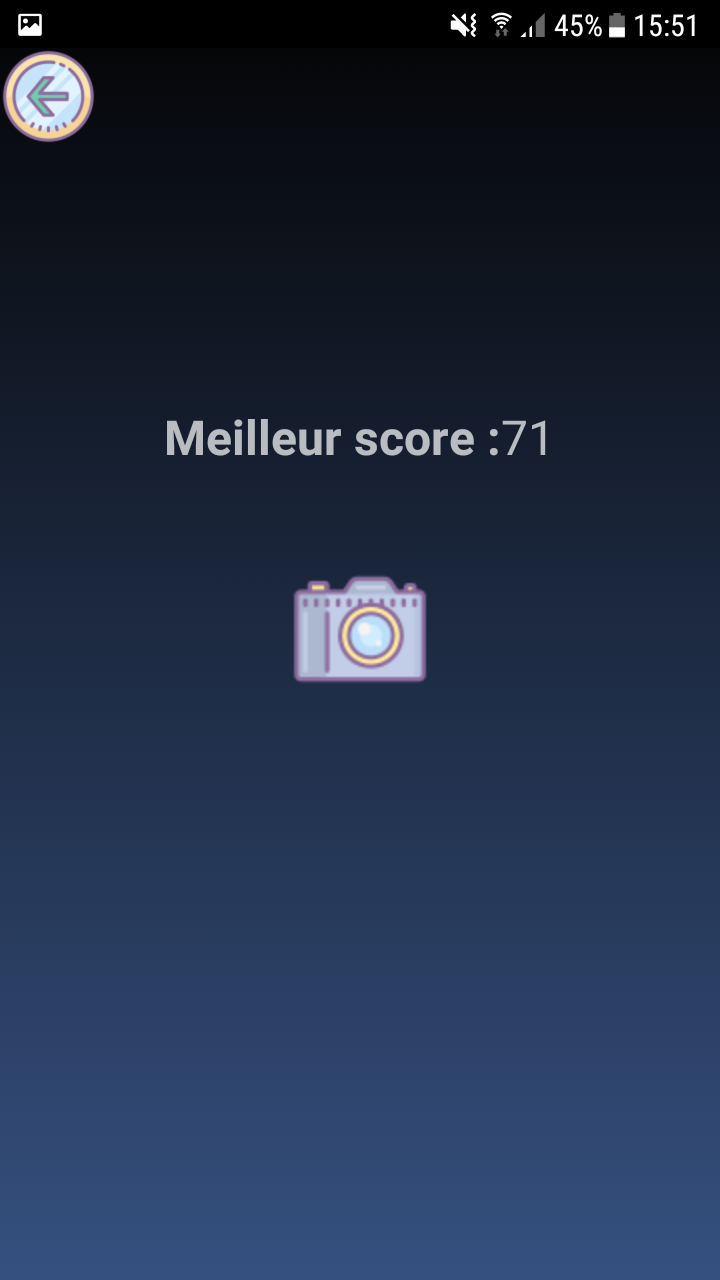
\includegraphics[scale = 0.18]{images/Android_1.png}
    \captionof{figure}{Gauche: Menu et Droite: Score}
\end{center}

\newpage
\subsubsection{L'interface de géo-localisation}
A la fin de chaque partie, le joueur aura la possibilité de visualiser sa position géographique.

\subsubsection{L'appareil photo}
Si le joueur le souhaite, nous avons intégré l'appareil photo pour qu'il puisse prendre un petit selfie pour se rappeler de sa victoire.\\

Voir ci-dessous les images correspondantes:

\begin{center}
    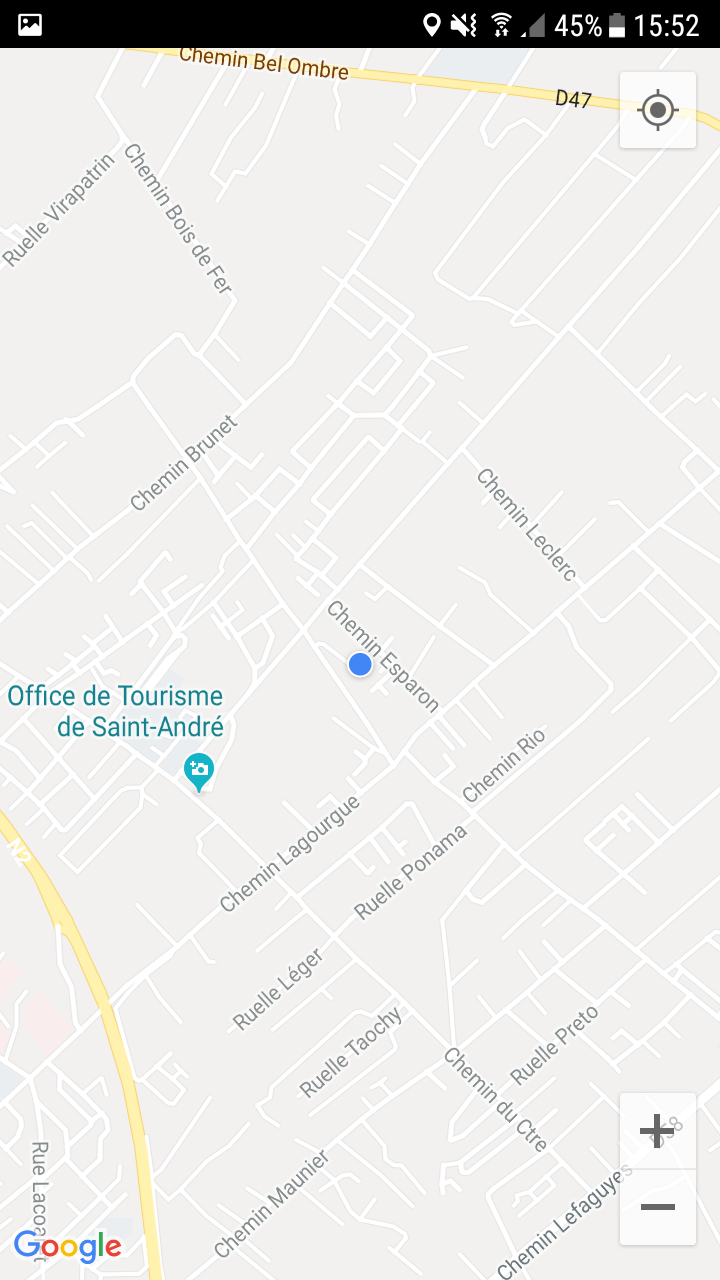
\includegraphics[scale = 0.18]{images/Android_2.png}
    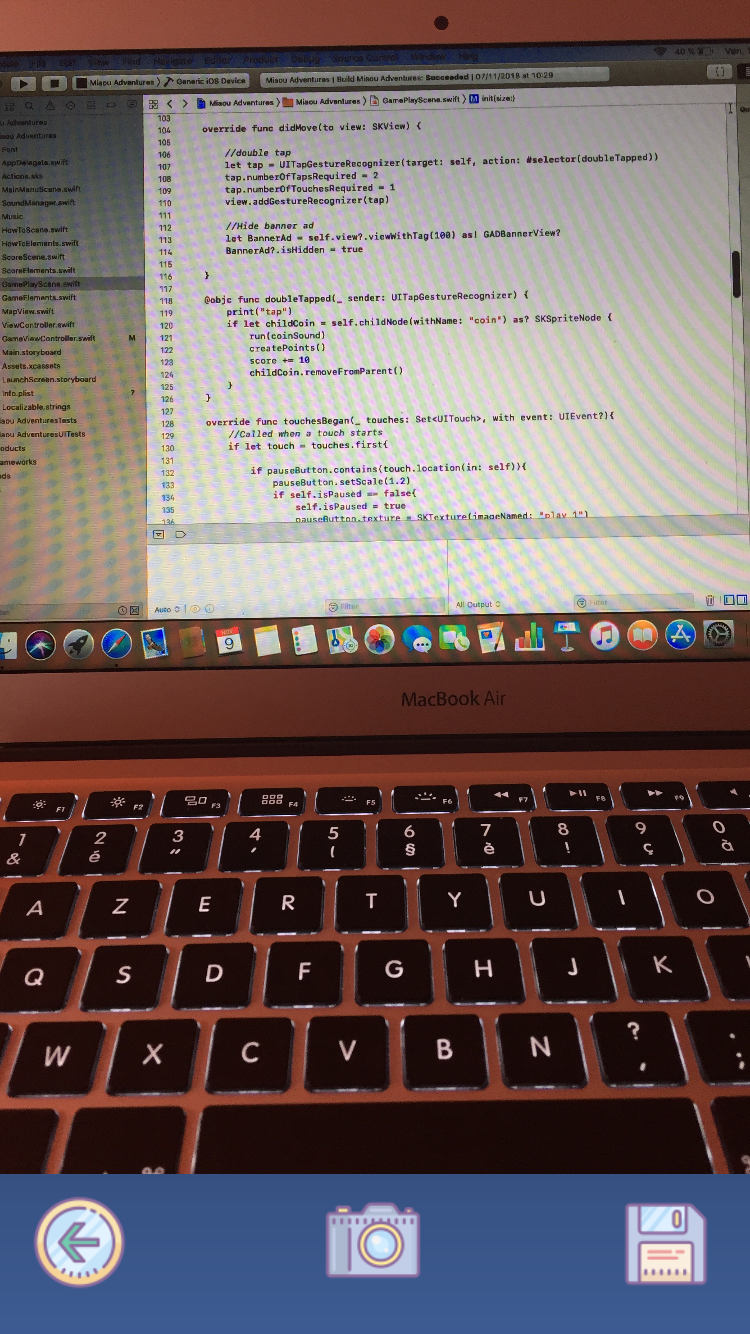
\includegraphics[scale = 0.18]{images/iOS_2.PNG}
    \captionof{figure}{Gauche: Géo-localisation et Droite: Appareil photo}
\end{center}

\newpage
\subsubsection{L'interface de jeu}
Sur l'interface de jeu, on retrouve tous les éléments de jeu. C'est la scène principale où le joueur prend contrôle de son vaisseau. Le but est simple, aller le plus loin possible en évitant les obstacles et récupérer les points bonus. L'utilisateur a la possibilité de quitter la partie en cours, de faire pause ou de redémarrer une partie. 
\subsubsection{Défaite du joueur}
Lorsque le joueur perd, le Game Over apparaît. Sur cette partie, le jeu affiche votre score. On retrouve également les boutons pour quitter le jeu, redémarrer une partie ou afficher sa position actuelle.\\

Voir ci-dessous les images correspondantes:

\begin{center}
    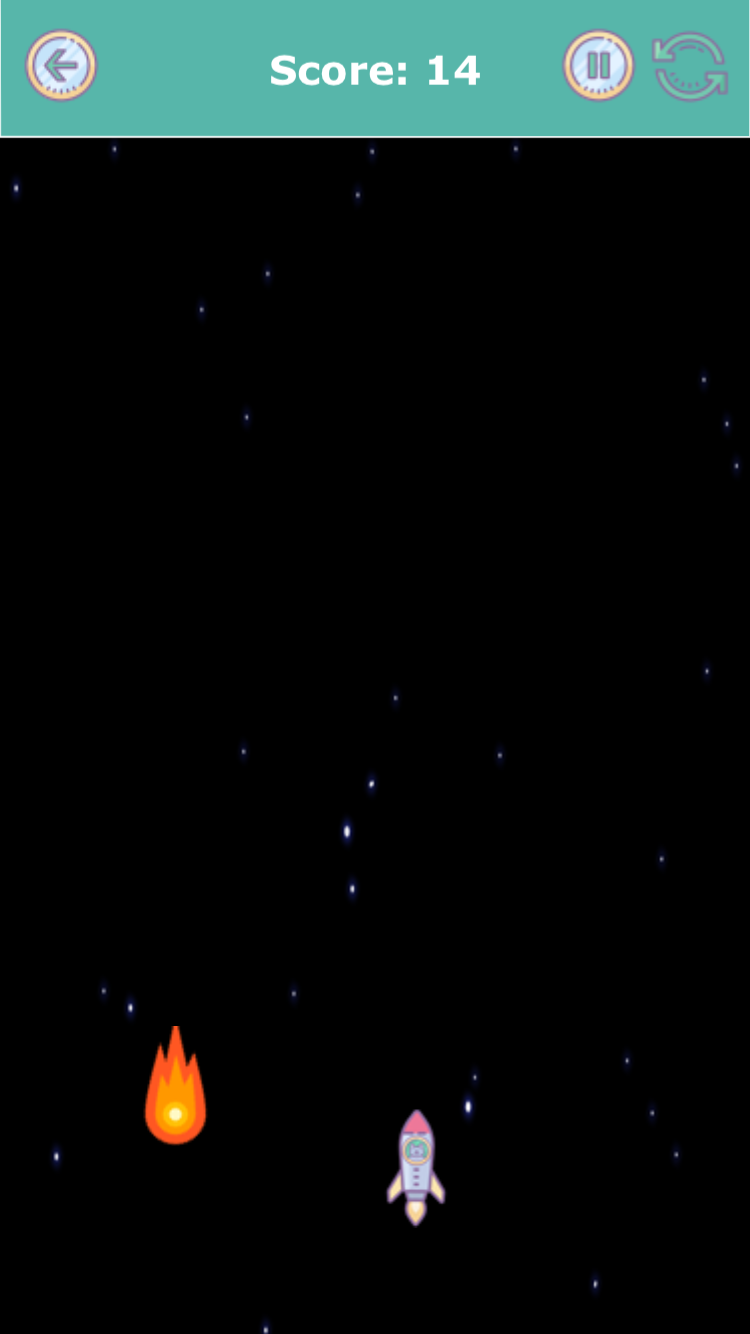
\includegraphics[scale = 0.18]{images/iOS_3.PNG}
    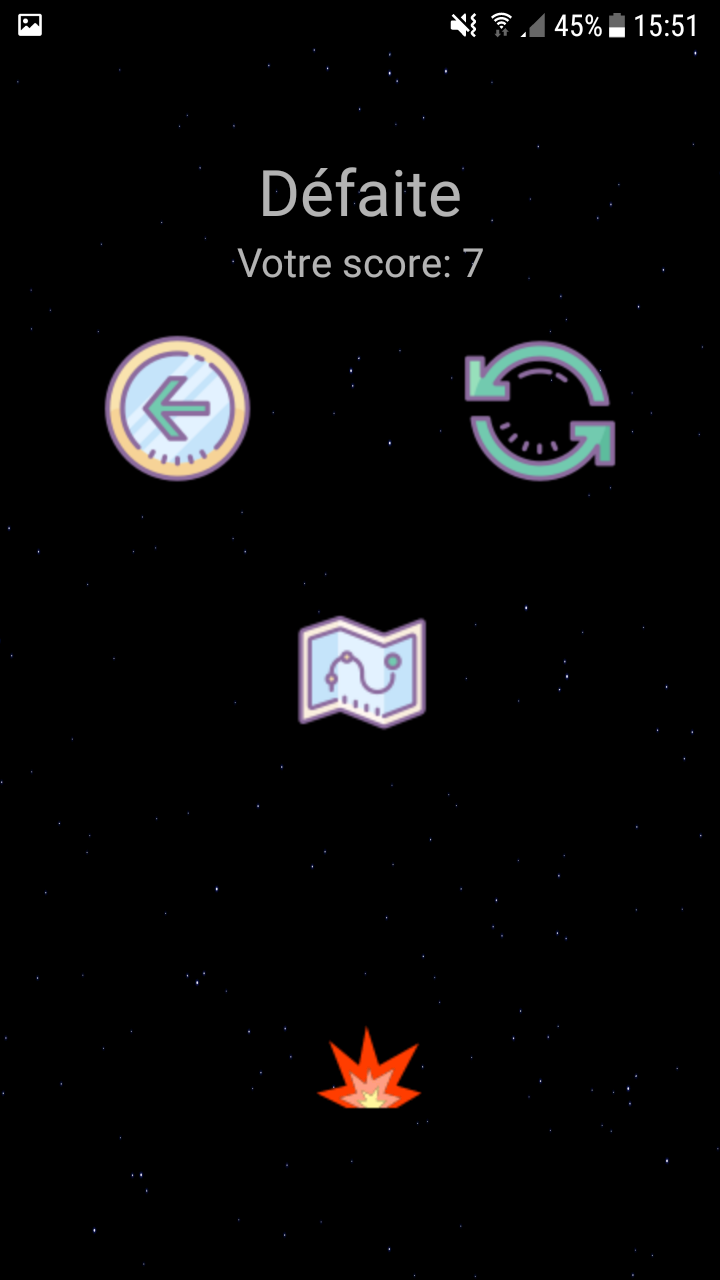
\includegraphics[scale = 0.18]{images/Android_3.png}
    \captionof{figure}{Gauche: Jeu et Droite: Fin de partie}
\end{center}

\newpage
\part*{Conclusion}
En conclusion, ce projet fut une belle épreuve qui nous a permis d’acquérir d'avantage d'expérience dans le développement d'applications pour mobiles.\\
L'année de L3 nous a permis d'emmagasiner de nombreuses connaissances. c
Cette année de Master, par contre, nous a permis d'améliorer nos compétences à travers la pratique. Notre savoir a été mis en application en situation réelle. 
Sur le plan personnel, il a été très fructueux de travailler en équipe. Nous avons pu créer une véritable cohésion et mettre en place un dialogue. Ce projet nous a permis de confronter nos idées, développer notre esprit d'équipe, d'améliorer nos capacités rédactionnelles et de mettre de côté nos différents et idées antagonistes afin de pouvoir créer le meilleur jeu possible.\\

Petit remerciement aux sites: Icons8 \cite{Icons8} et Zapsplat \cite{Zapsplat} pour nous avoir fourni les sprites et les sons.


\newpage
\bibliographystyle{unsrt}
\bibliography{bibli}

\end{document}
